\documentclass[border=4pt,12pt]{standalone}
% House style for redrawn exam diagrams (diagram-v4: 0.4pt lines, filled -latex arrows, fine dashes; stipple and hatching drawn as real dots/lines (no PDF/SVG patterns, so they render in every browser and at any scale); transparent background). Every figure \input's this.
\usepackage{amsmath,amssymb}
\usepackage{txfonts}
\usepackage{pdfrender,xcolor}
% \halo{text}: label on shading. The shading stops just around each letter's outline (a thin knock-out that follows the
% glyphs, like the papers' typesetting), never a box. Owner: "I don't want a box around the text".
\newcommand{\halo}[1]{\leavevmode\rlap{\pdfrender{TextRenderingMode=2,LineWidth=2.2pt,LineJoinStyle=1,StrokeColor=white,FillColor=white}#1}#1}
\usepackage{tikz,pgfplots}
\pgfplotsset{compat=1.18}
\usetikzlibrary{arrows.meta,calc,angles,quotes,patterns,patterns.meta,intersections,positioning,decorations.markings,shapes.geometric}
% Stipple and hatching are drawn as actual dots / lines clipped to the region (path picture), NOT as pattern fills:
% SVG <pattern> fills vanish or blur when browsers scale the image, so the owner could not see the shading.
% Each dot is a 0.72pt square (keeps SVGs small; reads as a dot at print size). Dots sit on one global staggered grid, so neighbouring regions line up.
\makeatletter
\newdimen\ex@x \newdimen\ex@y \newdimen\ex@xa \newdimen\ex@ya \newdimen\ex@xb \newdimen\ex@yb \newcount\ex@row
\def\exam@stipplecolor{black!75}\def\exam@dotr{0.42pt}\def\exam@dotgap{2.5}
\def\ex@rowdots{\ifdim\ex@x<\ex@xb \pgfpathrectangle{\pgfqpoint{\dimexpr\ex@x-0.36pt\relax}{\dimexpr\ex@y-0.36pt\relax}}{\pgfqpoint{0.72pt}{0.72pt}}\advance\ex@x by \exam@dotgap pt\relax\expandafter\ex@rowdots\fi}
\def\exam@stipple{%
  \pgftransformreset% dots are sized in real points even inside scaled pictures
  \pgfpointanchor{path picture bounding box}{south west}\ex@xa=\pgf@x \ex@ya=\pgf@y
  \pgfpointanchor{path picture bounding box}{north east}\ex@xb=\pgf@x \ex@yb=\pgf@y
  \pgfsetfillcolor{\exam@stipplecolor}\pgfmathsetmacro\ex@h{\exam@dotgap/2}%
  \pgfmathtruncatemacro\ex@r{floor(\ex@ya/\ex@h)-1}\ex@row=\ex@r\relax
  \ex@y=\ex@r\dimexpr\ex@h pt\relax
  \loop\ifdim\ex@y<\ex@yb
    \pgfmathtruncatemacro\ex@c{floor(\ex@xa/\exam@dotgap)-1}\ex@x=\ex@c\dimexpr\exam@dotgap pt\relax
    \ifodd\ex@row \advance\ex@x by \ex@h pt\fi
    \ex@rowdots
    \advance\ex@y by \ex@h pt \advance\ex@row by 1
    \ifnum\numexpr\ex@row-(\ex@row/4)*4\relax=0 \pgfusepath{fill}\fi% flush every 4 rows: bounded TeX memory, few clip copies in the SVG
  \repeat\pgfusepath{fill}}
\newdimen\ex@d
\def\exam@hatch#1{% #1 = 1 for /, -1 for \ ; lines 45 degrees, 3pt apart
  \pgftransformreset
  \pgfpointanchor{path picture bounding box}{south west}\ex@xa=\pgf@x \ex@ya=\pgf@y
  \pgfpointanchor{path picture bounding box}{north east}\ex@xb=\pgf@x \ex@yb=\pgf@y
  \ex@d=\dimexpr\ex@yb-\ex@ya\relax \ex@x=\dimexpr\ex@xa-\ex@d\relax
  \loop\ifdim\ex@x<\ex@xb
    \ifnum#1>0 \pgfpathmoveto{\pgfqpoint{\ex@x}{\ex@ya}}\pgfpathlineto{\pgfqpoint{\dimexpr\ex@x+\ex@d\relax}{\ex@yb}}%
    \else \pgfpathmoveto{\pgfqpoint{\ex@x}{\ex@yb}}\pgfpathlineto{\pgfqpoint{\dimexpr\ex@x+\ex@d\relax}{\ex@ya}}\fi
    \advance\ex@x by 4.24pt
  \repeat
  \pgfsetlinewidth{0.4pt}\pgfsetstrokecolor{black}\pgfusepath{stroke}}
\def\examstipple{\exam@stipple}\def\examhatch{\exam@hatch}\def\examsetstipplecolor#1{\def\exam@stipplecolor{#1}}\def\examsetdotgap#1{\def\exam@dotgap{#1}}
\makeatother
% (legacy pattern kept for old files)
% staggered stipple like the NESA papers' dotted shading
\pgfdeclarepatternformonly{exam stipple}{\pgfpointorigin}{\pgfqpoint{2.2pt}{2.2pt}}{\pgfqpoint{2.2pt}{2.2pt}}{%
  \pgfpathcircle{\pgfqpoint{0.55pt}{0.55pt}}{0.42pt}\pgfpathcircle{\pgfqpoint{1.65pt}{1.65pt}}{0.42pt}\pgfusepath{fill}}
\tikzset{
  every picture/.style={line width=0.6pt, >={Latex[length=2mm,width=1.3mm]}},
  curve/.style={line width=0.6pt},
  open arrow/.style={-{Latex[length=2mm,width=1.3mm]}},  % owner: filled -latex heads everywhere, no open chevrons
  aux/.style={dash pattern=on 2pt off 1.5pt, line width=0.6pt},
  shade/.code={\def\exA{#1}\def\exB{none}\ifx\exA\exB\else\pgfkeysalso{fill=black!18}\fi},
  shade/.default=on,
  shade dots/.style={fill=none, path picture={\examstipple}},
  stipple color/.code={\examsetstipplecolor{#1}},
  stipple gap/.code={\examsetdotgap{#1}},
  shade dense dots/.style={fill=none, stipple gap=1.6, path picture={\examstipple}},
  shade hatch/.style={fill=none, path picture={\examhatch{1}}},
  shade hatch reverse/.style={fill=none, path picture={\examhatch{-1}}},
  shade solid/.style={fill=black},
  pt/.style={circle, fill, inner sep=1.1pt},
  open pt/.style={circle, draw, fill=white, inner sep=1.1pt},
}
\pgfplotsset{
  exam axes/.style={axis lines=middle, axis line style={->}, xlabel={$x$}, ylabel={$y$},
    xlabel style={anchor=west}, ylabel style={anchor=south}, tick label style={font=\small},
    every axis plot/.append style={line width=0.6pt, black}, samples=200, clip=false,
    enlargelimits=false, axis on top},
}

\begin{document}
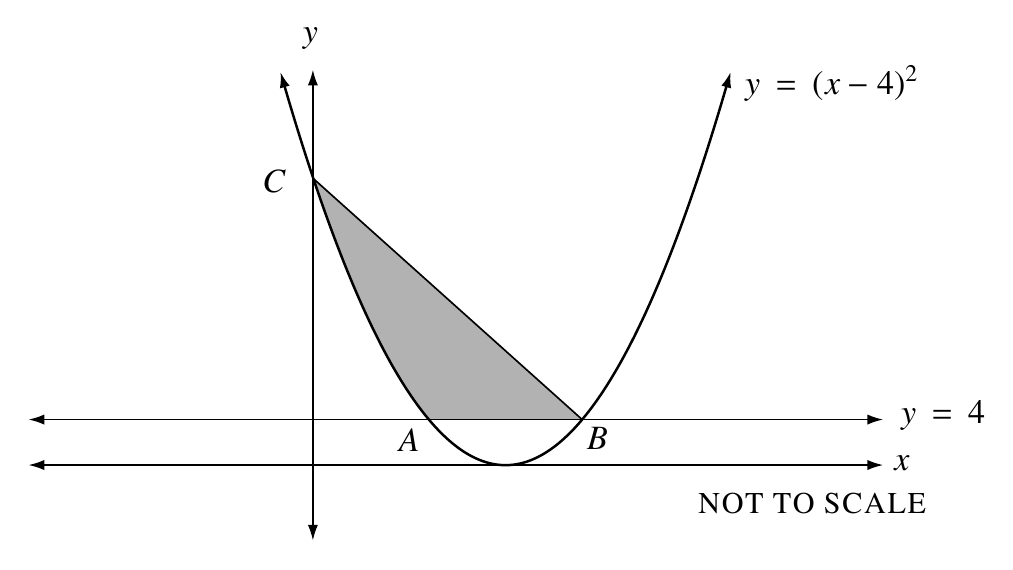
\begin{tikzpicture}[x=0.0127cm,y=-0.0127cm,every node/.style={font=\fontsize{12.3}{14.76}\selectfont}]
\fill[black!30] plot[smooth] coordinates {(315.00,187.02) (317.96,195.78) (320.92,204.41) (323.88,212.90) (326.85,221.26) (329.81,229.48) (332.77,237.56) (335.73,245.51) (338.69,253.32) (341.65,261.00) (344.62,268.54) (347.58,275.94) (350.54,283.21) (353.50,290.34) (356.46,297.34) (359.42,304.20) (362.38,310.92) (365.35,317.51) (368.31,323.96) (371.27,330.27) (374.23,336.45) (377.19,342.49) (380.15,348.40) (383.12,354.17) (386.08,359.80) (389.04,365.30) (392.00,370.66) (394.96,375.89) (397.92,380.98) (400.88,385.93) (403.85,390.75) (406.81,395.43) (409.77,399.98) (412.73,404.39) (415.69,408.66) (418.65,412.80) (421.62,416.80) (424.58,420.66) (427.54,424.39) (430.50,427.99)} -- (583.9,428) -- cycle;
\draw[<->] (30,473.5) -- (885,473.5);
\draw[<->] (314.5,549) -- (314.5,78);
\draw[<->] (30,428) -- (885,428);
\draw[<->,line width=0.9pt] plot[smooth] coordinates {(282.00,80.15) (287.06,97.63) (292.12,114.72) (297.18,131.41) (302.24,147.71) (307.30,163.60) (312.36,179.10) (317.42,194.20) (322.49,208.91) (327.55,223.21) (332.61,237.12) (337.67,250.63) (342.73,263.75) (347.79,276.47) (352.85,288.79) (357.91,300.71) (362.97,312.23) (368.03,323.36) (373.09,334.09) (378.15,344.42) (383.21,354.36) (388.27,363.90) (393.33,373.04) (398.40,381.78) (403.46,390.12) (408.52,398.07) (413.58,405.62) (418.64,412.78) (423.70,419.53) (428.76,425.89) (433.82,431.85) (438.88,437.42) (443.94,442.58) (449.00,447.35) (454.06,451.72) (459.12,455.70) (464.18,459.27) (469.24,462.45) (474.31,465.23) (479.37,467.62) (484.43,469.61) (489.49,471.20) (494.55,472.39) (499.61,473.18) (504.67,473.58) (509.73,473.58) (514.79,473.18) (519.85,472.39) (524.91,471.20) (529.97,469.61) (535.03,467.62) (540.09,465.23) (545.16,462.45) (550.22,459.27) (555.28,455.70) (560.34,451.72) (565.40,447.35) (570.46,442.58) (575.52,437.42) (580.58,431.85) (585.64,425.89) (590.70,419.53) (595.76,412.78) (600.82,405.62) (605.88,398.07) (610.94,390.12) (616.00,381.78) (621.07,373.04) (626.13,363.90) (631.19,354.36) (636.25,344.42) (641.31,334.09) (646.37,323.36) (651.43,312.23) (656.49,300.71) (661.55,288.79) (666.61,276.47) (671.67,263.75) (676.73,250.63) (681.79,237.12) (686.85,223.21) (691.91,208.91) (696.98,194.20) (702.04,179.10) (707.10,163.60) (712.16,147.71) (717.22,131.41) (722.28,114.72) (727.34,97.63) (732.40,80.15)};
\draw (315,187.02) -- (583.9,428);
\node[inner sep=0] at (276.5,190) {$C$};
\node[inner sep=0] at (410.5,449) {$A$};
\node[inner sep=0] at (598.5,446.5) {$B$};
\node[inner sep=0] at (312,47) {$y$};
\node[inner sep=0] at (903,472) {$x$};
\node[inner sep=0] at (945,424) {$y\,=\,4$};
\node[inner sep=0,anchor=west] at (746,92) {$y\,=\,(x-4)^2$};
\node[inner sep=0] at (814,512) {\fontsize{10.9}{13}\selectfont N\kern.6pt O\kern.6pt T\kern.6pt\ T\kern.6pt O\kern.6pt\ S\kern.6pt C\kern.6pt A\kern.6pt L\kern.6pt E};
\end{tikzpicture}
\end{document}
